\tikzstyle{title} = [text width=7em]
\tikzstyle{input} = [rectangle, draw,
    text width=2em, text centered, rounded corners, node distance=1cm, minimum height=1.6em]
\tikzstyle{embed} = [rectangle, draw,
    text width=2em, text centered, node distance=1cm, minimum height=1.6em]
\tikzstyle{plus} = [text width=2em, text centered, node distance=1cm]
% \tikzstyle{line} = [draw, -latex']
% \tikzstyle{cloud} = [draw, ellipse, node distance=3cm,
%     text width=5em, text centered, minimum height=2em]

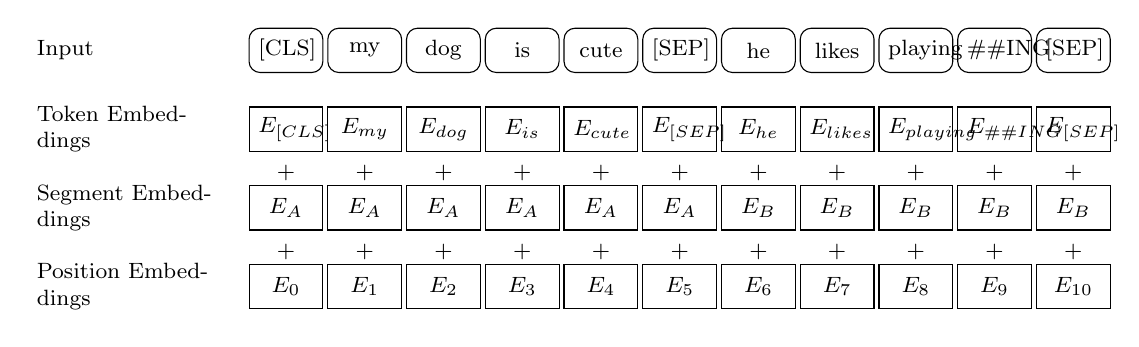
\begin{tikzpicture}[font=\footnotesize]
\node [title] (i-1) {Input};
\node [input, right of=i-1, node distance=5.5em] (i0) {[CLS]};
\node [input, right of=i0] (i1) {my};
\node [input, right of=i1] (i2) {dog};
\node [input, right of=i2] (i3) {is};
\node [input, right of=i3] (i4) {cute};
\node [input, right of=i4] (i5) {[SEP]};
\node [input, right of=i5] (i6) {he};
\node [input, right of=i6] (i7) {likes};
\node [input, right of=i7] (i8) {playing};
\node [input, right of=i8] (i9) {\#\#ING};
\node [input, right of=i9] (i10) {[SEP]};

\node [title, below of=i-1] (te-1) {Token Embeddings};
\node [embed, right of=te-1, node distance=5.5em] (te0) {$\text{E}_{\text{[CLS]}}$};
\node [embed, right of=te0] (te1) {$\text{E}_{\text{my}}$};
\node [embed, right of=te1] (te2) {$\text{E}_{\text{dog}}$};
\node [embed, right of=te2] (te3) {$\text{E}_{\text{is}}$};
\node [embed, right of=te3] (te4) {$\text{E}_{\text{cute}}$};
\node [embed, right of=te4] (te5) {$\text{E}_{\text{[SEP]}}$};
\node [embed, right of=te5] (te6) {$\text{E}_{\text{he}}$};
\node [embed, right of=te6] (te7) {$\text{E}_{\text{likes}}$};
\node [embed, right of=te7] (te8) {$\text{E}_{\text{playing}}$};
\node [embed, right of=te8] (te9) {$\text{E}_{\text{\#\#ING}}$};
\node [embed, right of=te9] (te10) {$\text{E}_{\text{[SEP]}}$};

\node [title, below of=te-1] (se-1) {Segment Embeddings};
\node [embed, right of=se-1, node distance=5.5em] (se0) {$\text{E}_{\text{A}}$};
\node [embed, right of=se0] (se1) {$\text{E}_{\text{A}}$};
\node [embed, right of=se1] (se2) {$\text{E}_{\text{A}}$};
\node [embed, right of=se2] (se3) {$\text{E}_{\text{A}}$};
\node [embed, right of=se3] (se4) {$\text{E}_{\text{A}}$};
\node [embed, right of=se4] (se5) {$\text{E}_{\text{A}}$};
\node [embed, right of=se5] (se6) {$\text{E}_{\text{B}}$};
\node [embed, right of=se6] (se7) {$\text{E}_{\text{B}}$};
\node [embed, right of=se7] (se8) {$\text{E}_{\text{B}}$};
\node [embed, right of=se8] (se9) {$\text{E}_{\text{B}}$};
\node [embed, right of=se9] (se10) {$\text{E}_{\text{B}}$};

\node [title, below of=se-1] (pe-1) {Position Embeddings};
\node [embed, right of=pe-1, node distance=5.5em] (pe0) {$\text{E}_{\text{0}}$};
\node [embed, right of=pe0] (pe1) {$\text{E}_{\text{1}}$};
\node [embed, right of=pe1] (pe2) {$\text{E}_{\text{2}}$};
\node [embed, right of=pe2] (pe3) {$\text{E}_{\text{3}}$};
\node [embed, right of=pe3] (pe4) {$\text{E}_{\text{4}}$};
\node [embed, right of=pe4] (pe5) {$\text{E}_{\text{5}}$};
\node [embed, right of=pe5] (pe6) {$\text{E}_{\text{6}}$};
\node [embed, right of=pe6] (pe7) {$\text{E}_{\text{7}}$};
\node [embed, right of=pe7] (pe8) {$\text{E}_{\text{8}}$};
\node [embed, right of=pe8] (pe9) {$\text{E}_{\text{9}}$};
\node [embed, right of=pe9] (pe10) {$\text{E}_{\text{10}}$};

\node [title, below of=te-1, node distance=1.6em] (pA-1) {};
\node [plus, right of=pA-1, node distance=5.5em] (pA0) {+};
\node [plus, right of=pA0] (pA1) {+};
\node [plus, right of=pA1] (pA2) {+};
\node [plus, right of=pA2] (pA3) {+};
\node [plus, right of=pA3] (pA4) {+};
\node [plus, right of=pA4] (pA5) {+};
\node [plus, right of=pA5] (pA6) {+};
\node [plus, right of=pA6] (pA7) {+};
\node [plus, right of=pA7] (pA8) {+};
\node [plus, right of=pA8] (pA9) {+};
\node [plus, right of=pA9] (pA10) {+};

\node [title, below of=se-1, node distance=1.6em] (pB-1) {};
\node [plus, right of=pB-1, node distance=5.5em] (pB0) {+};
\node [plus, right of=pB0] (pB1) {+};
\node [plus, right of=pB1] (pB2) {+};
\node [plus, right of=pB2] (pB3) {+};
\node [plus, right of=pB3] (pB4) {+};
\node [plus, right of=pB4] (pB5) {+};
\node [plus, right of=pB5] (pB6) {+};
\node [plus, right of=pB6] (pB7) {+};
\node [plus, right of=pB7] (pB8) {+};
\node [plus, right of=pB8] (pB9) {+};
\node [plus, right of=pB9] (pB10) {+};

\end{tikzpicture}
